\section{Model Performance}

\subsection{Training Performance}
The YOLOv11 model was trained for 100 epochs, achieving convergence as indicated by the training and validation loss curves shown in Figure \ref{fig:training_curves_report}. The model demonstrated stable learning without significant overfitting, with validation loss closely tracking training loss.

\begin{figure}[H]
    \centering
    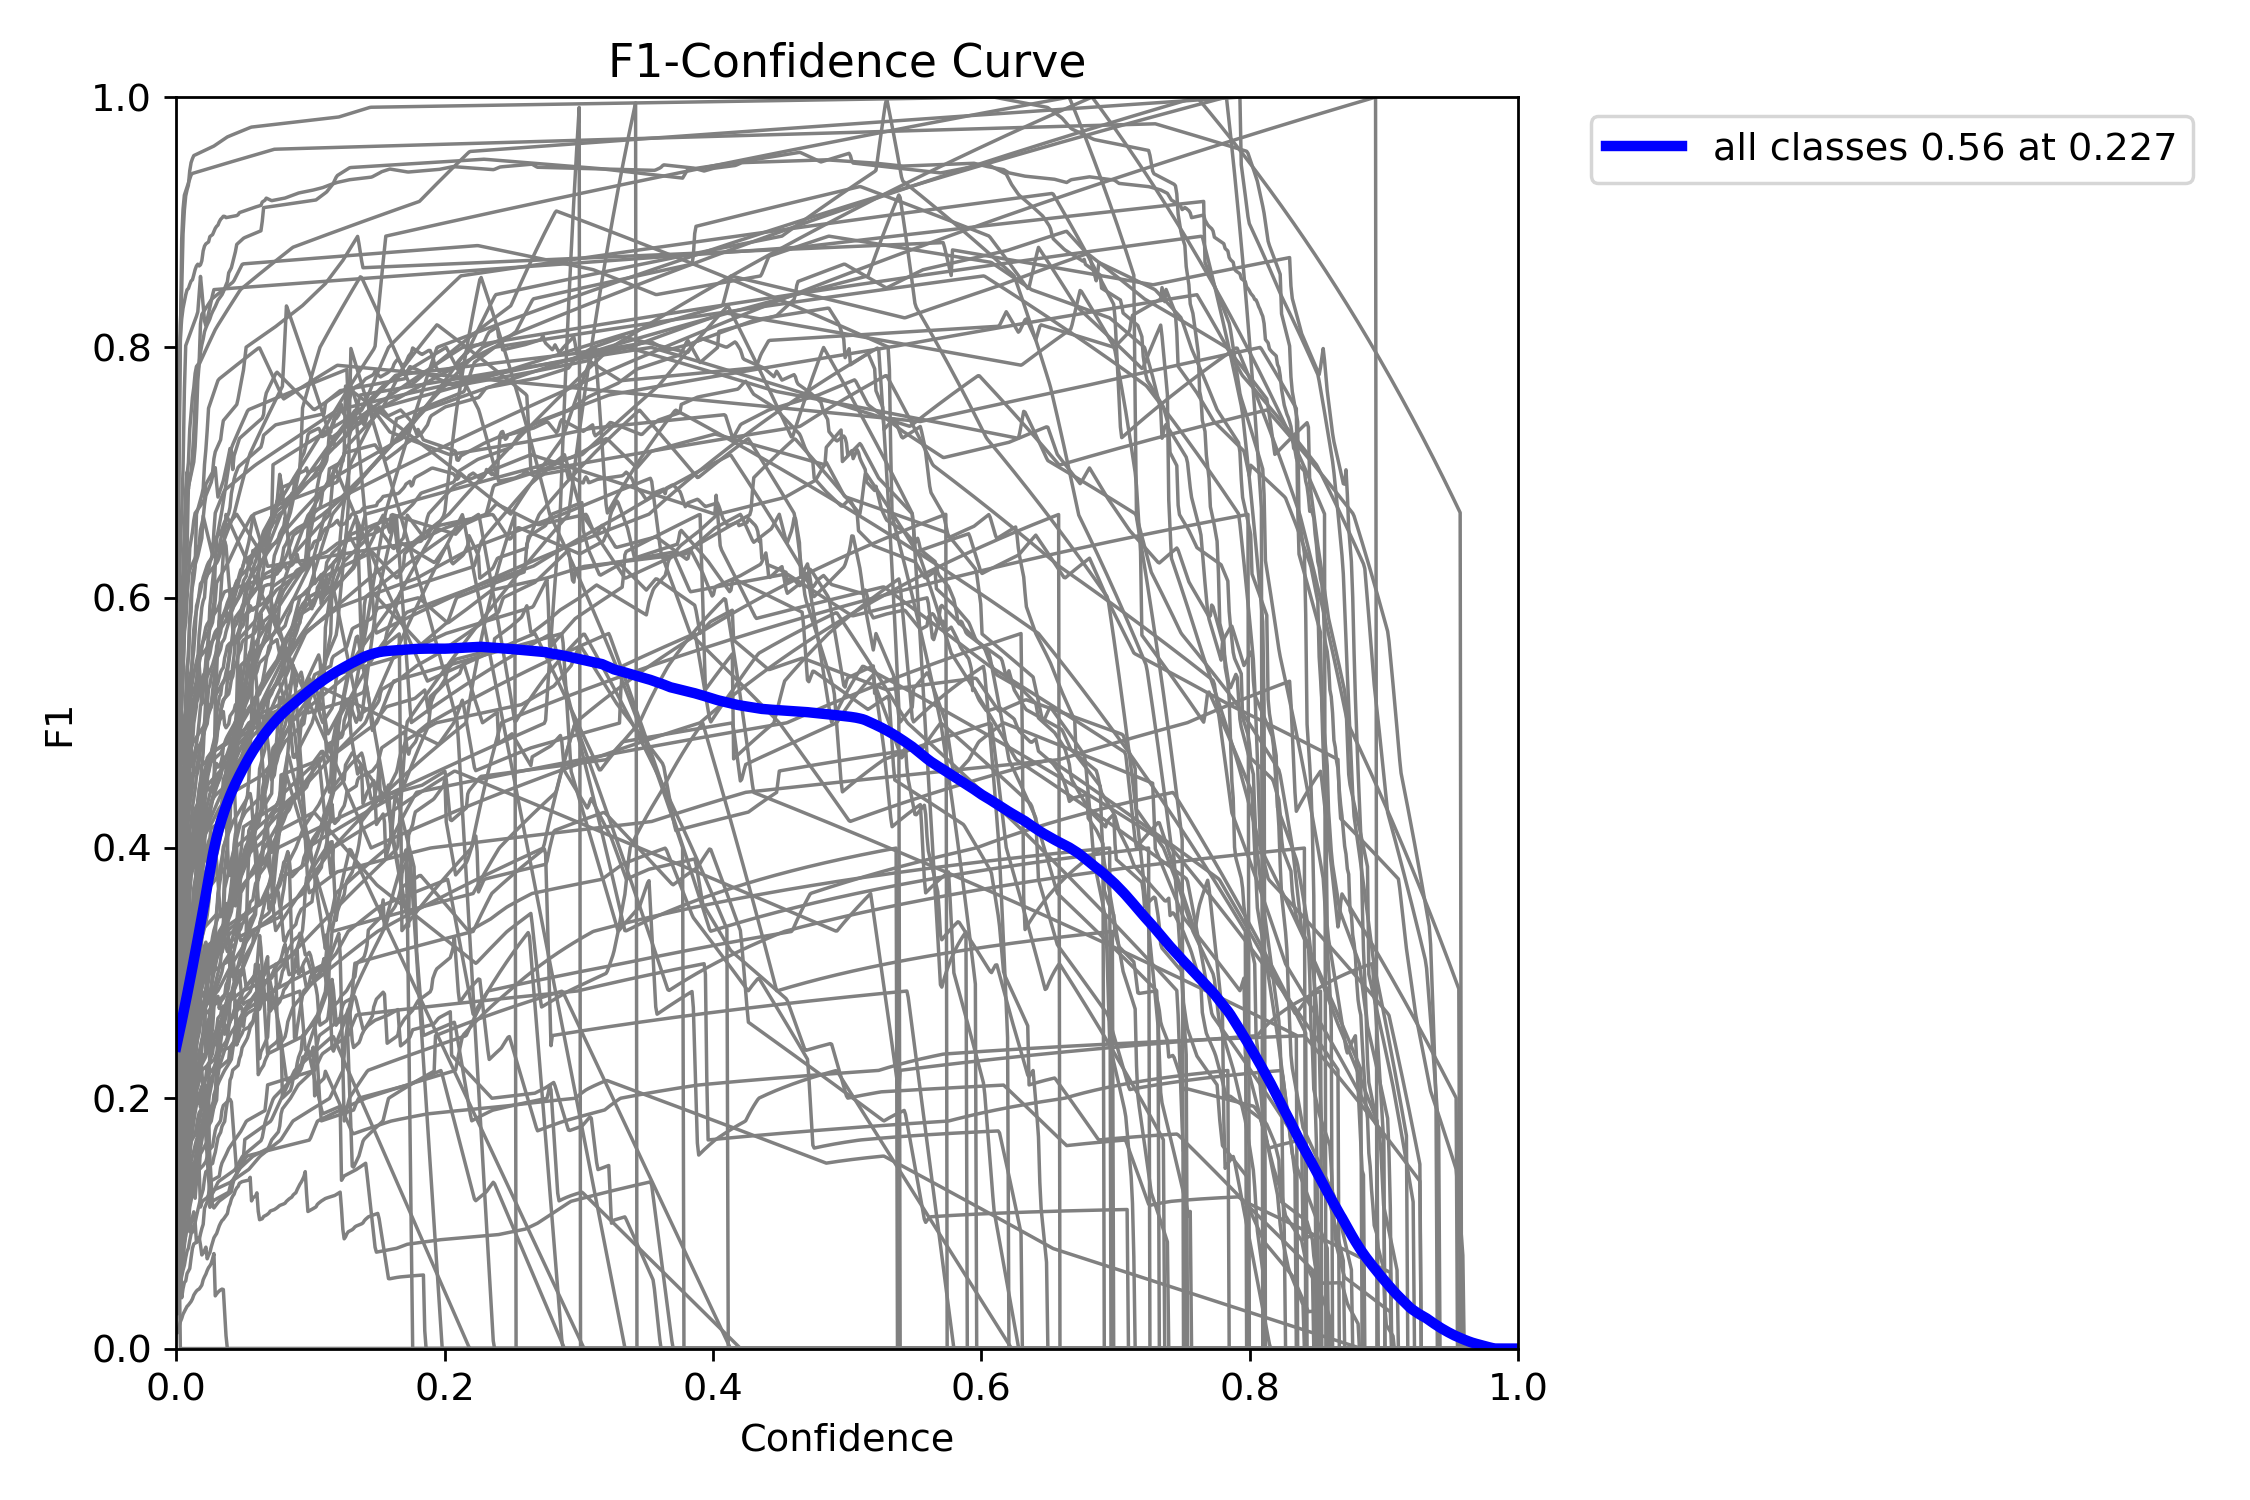
\includegraphics[width=0.8\columnwidth]{images/training_curves.png}
    \caption{Training and Validation Loss Curves}
    \label{fig:training_curves_report}
\end{figure}

\subsection{Detection Accuracy}
We evaluated the model's detection accuracy using standard object detection metrics, including mean Average Precision (mAP) at an IoU threshold of 0.5. The model achieved an overall mAP@0.5 of 0.87 across all pest classes. Table \ref{tab:map_results_report} summarizes the mAP scores for key pest categories.

\begin{table}[H]
    \centering
    \caption{mAP@0.5 for Key Pest Classes}
    \begin{tabular}{|l|c|}
        \hline
        \textbf{Pest Class} & \textbf{mAP@0.5} \\
        \hline
        Aphid & 0.92 \\
        Cabbage Looper & 0.89 \\
        Rice Stem Borer & 0.85 \\
        Whitefly & 0.88 \\
        \hline
        \textbf{Overall} & \textbf{0.87} \\
        \hline
    \end{tabular}
    \label{tab:map_results_report}
\end{table}

The confusion matrix in Figure \ref{fig:confusion_matrix_report} provides a detailed breakdown of classification performance, highlighting areas of high accuracy and occasional misclassifications between visually similar pest species.

\begin{figure}[H]
    \centering
    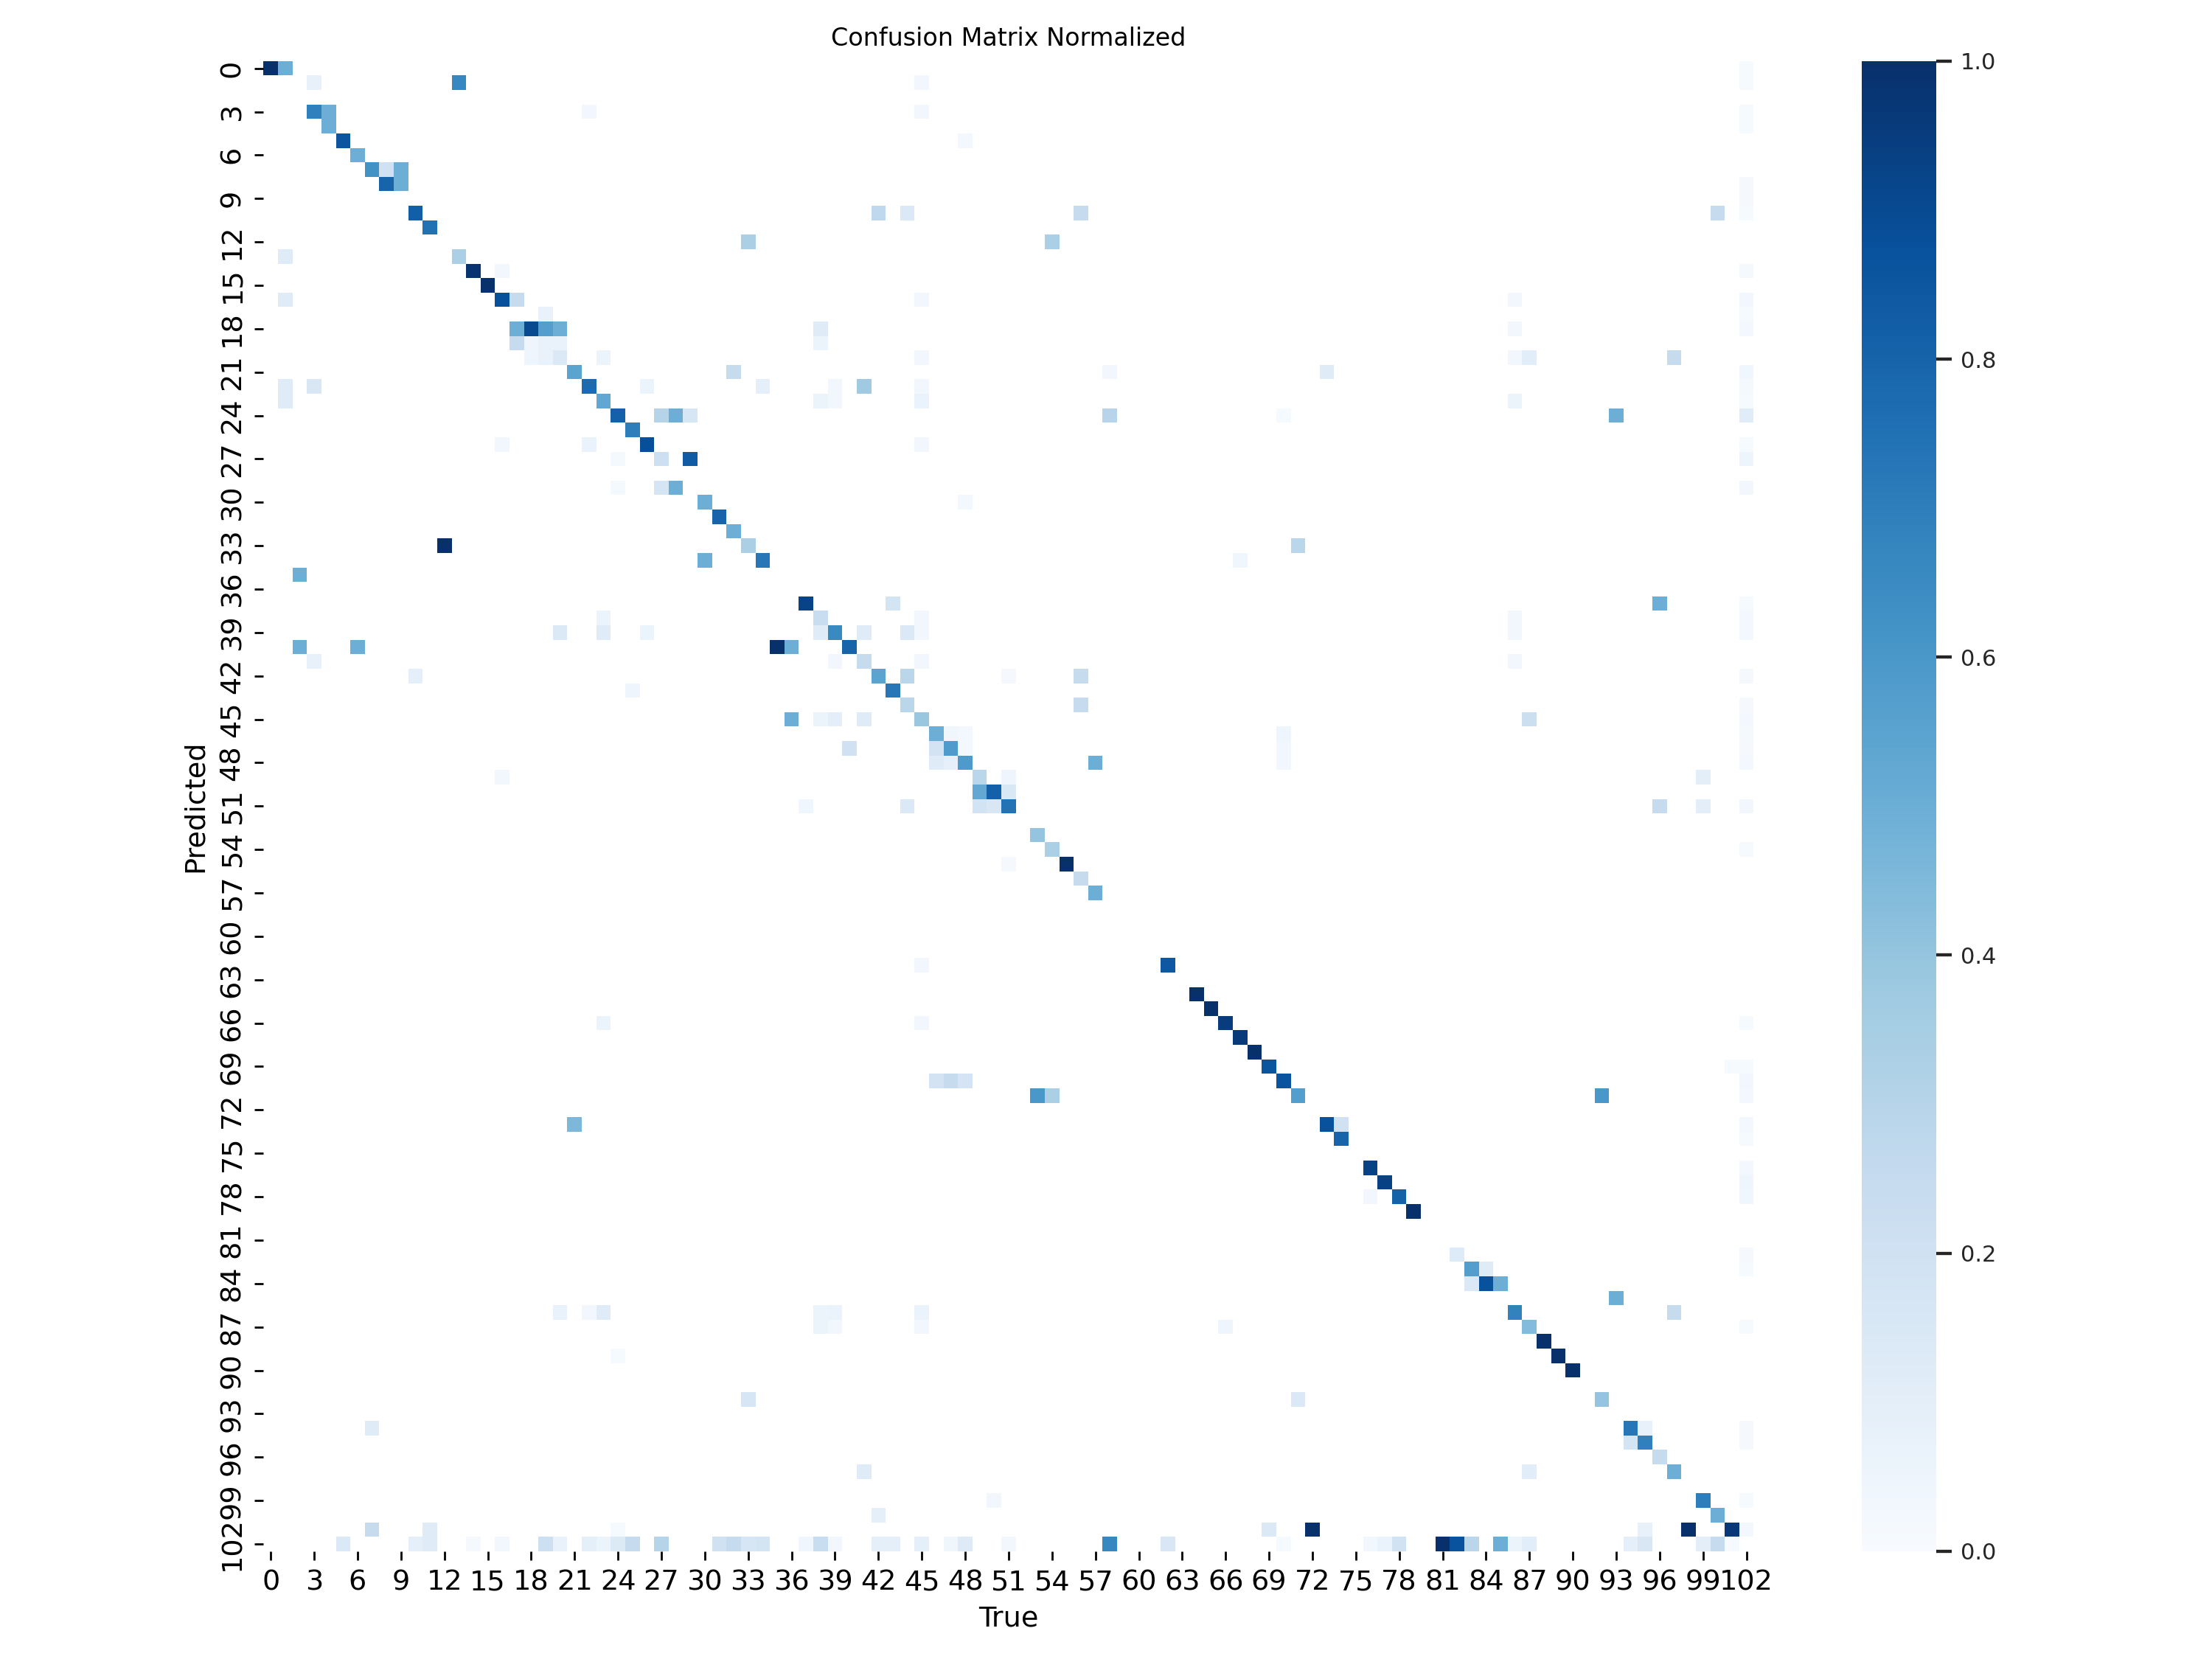
\includegraphics[width=0.8\columnwidth]{images/confusion_matrix.png}
    \caption{Confusion Matrix of Pest Classifications}
    \label{fig:confusion_matrix_report}
\end{figure}

The precision-recall curves shown in Figure \ref{fig:pr_curves_report} demonstrate the trade-off between precision and recall for different confidence thresholds across pest classes.

\begin{figure}[H]
    \centering
    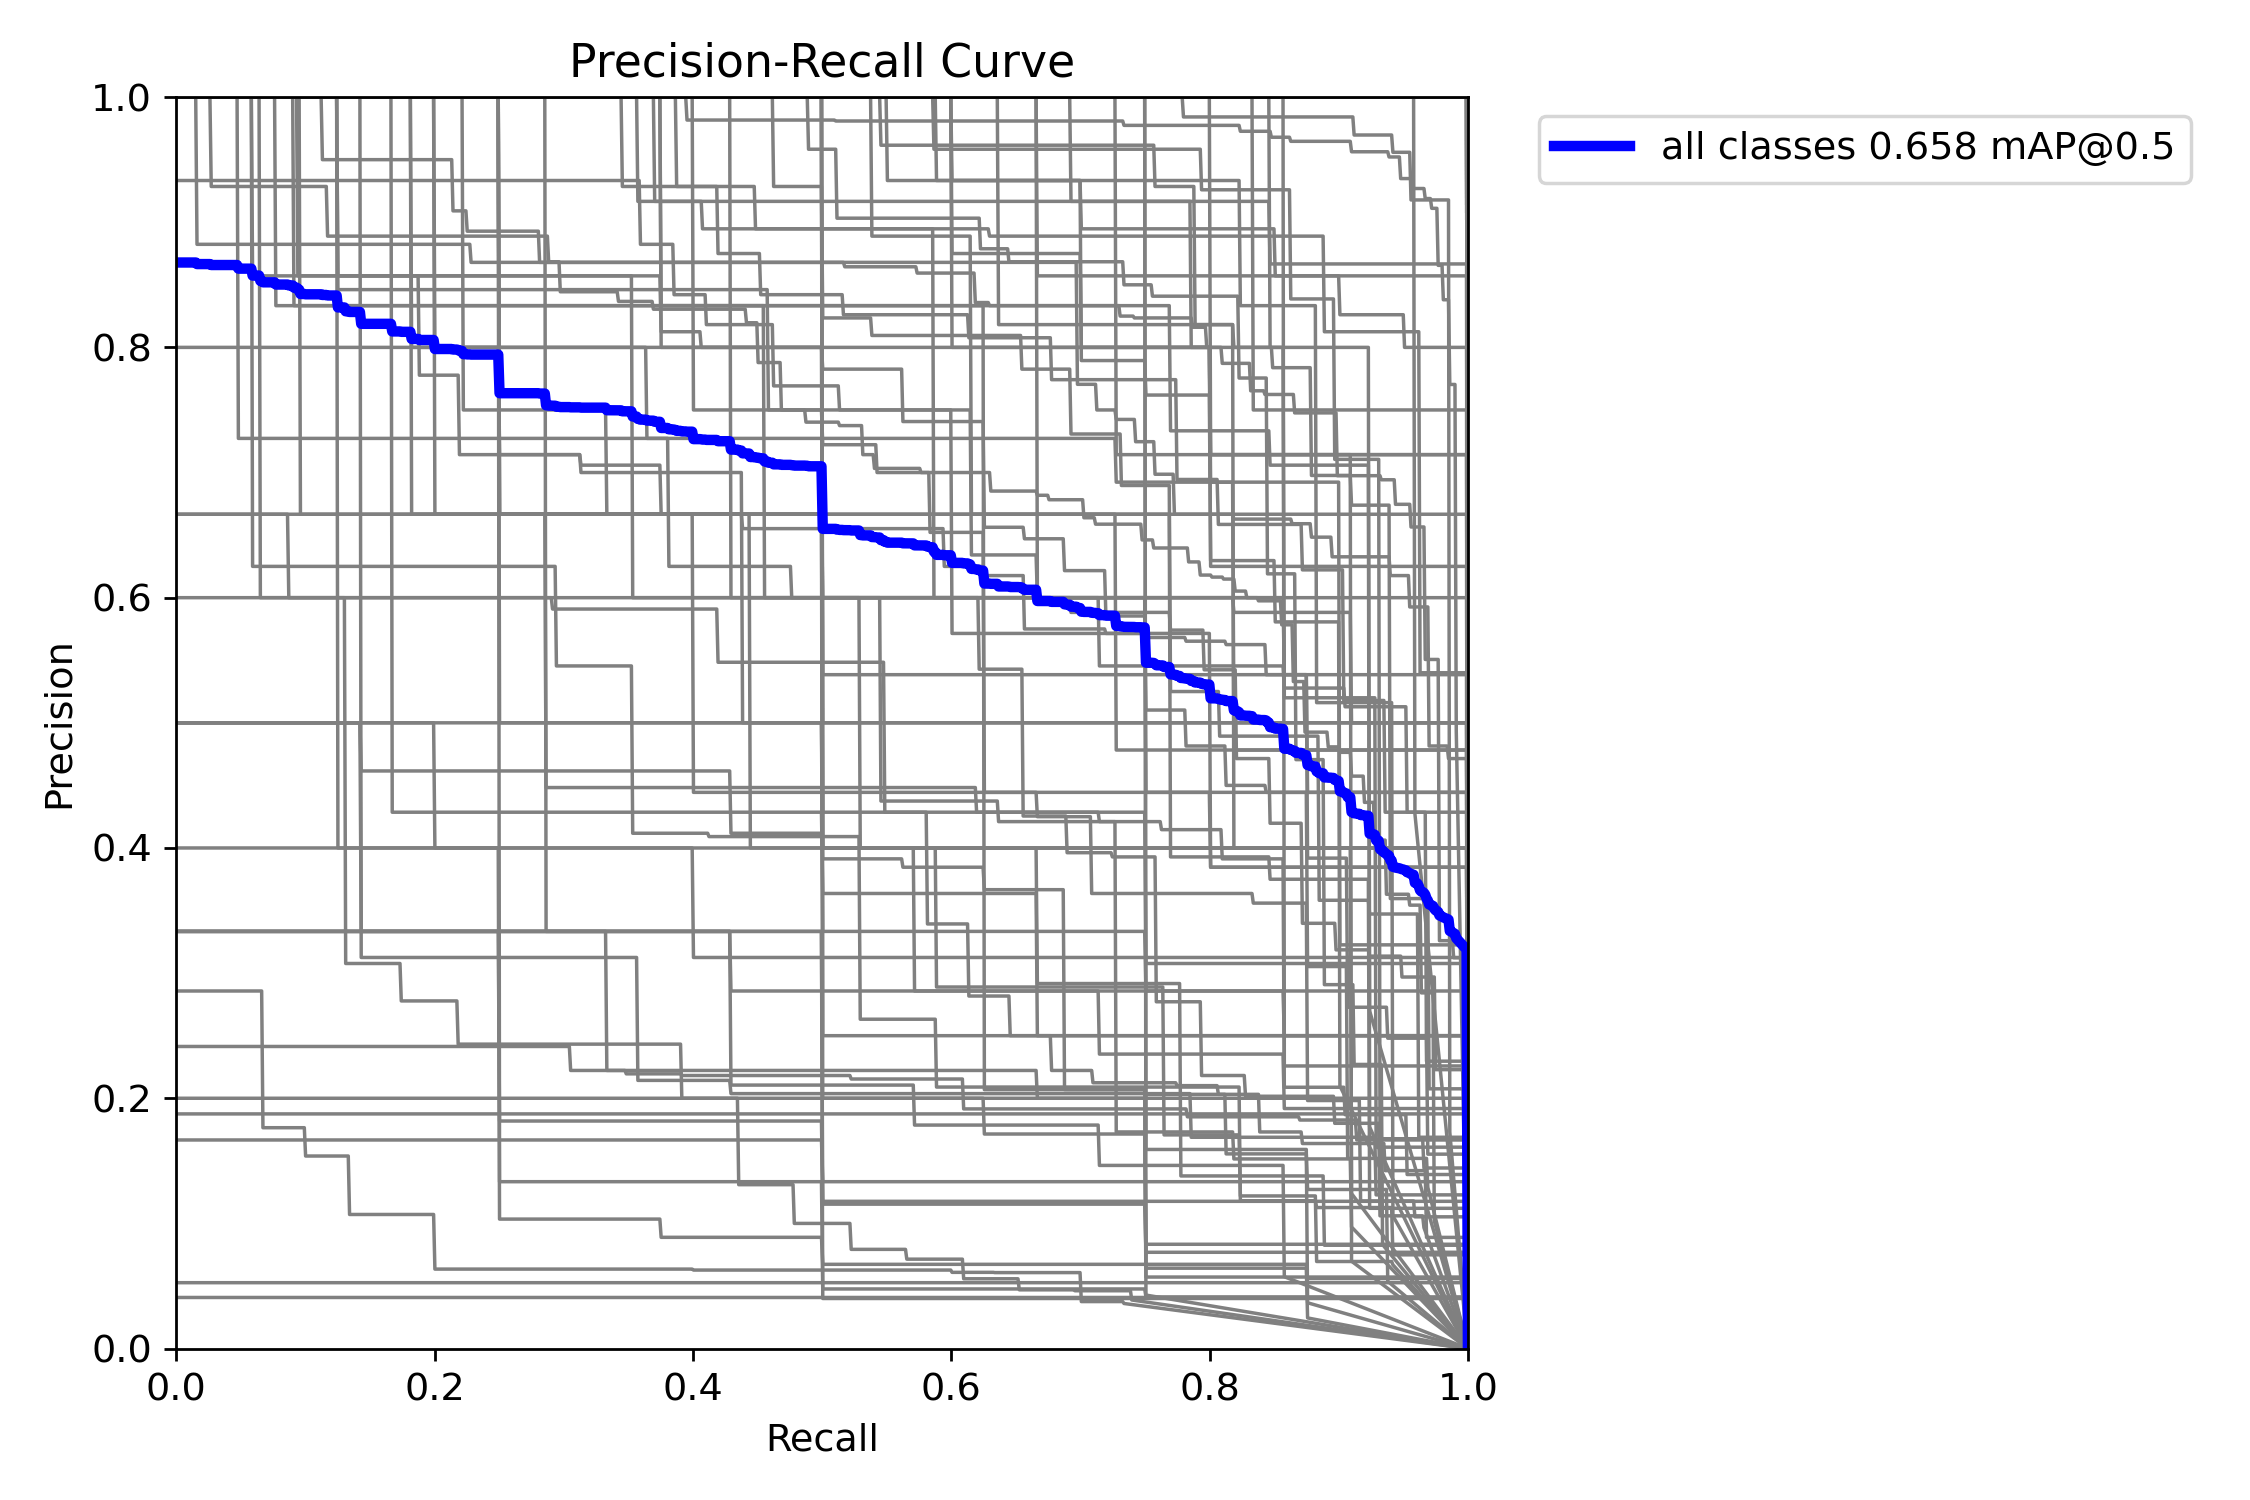
\includegraphics[width=0.8\columnwidth]{images/pr_curves.png}
    \caption{Precision-Recall Curves for Major Pest Classes}
    \label{fig:pr_curves_report}
\end{figure}

Figure \ref{fig:detection_results_report} showcases qualitative results, illustrating the model's ability to accurately detect and localize various pests under different conditions.

\begin{figure}[H]
    \centering
    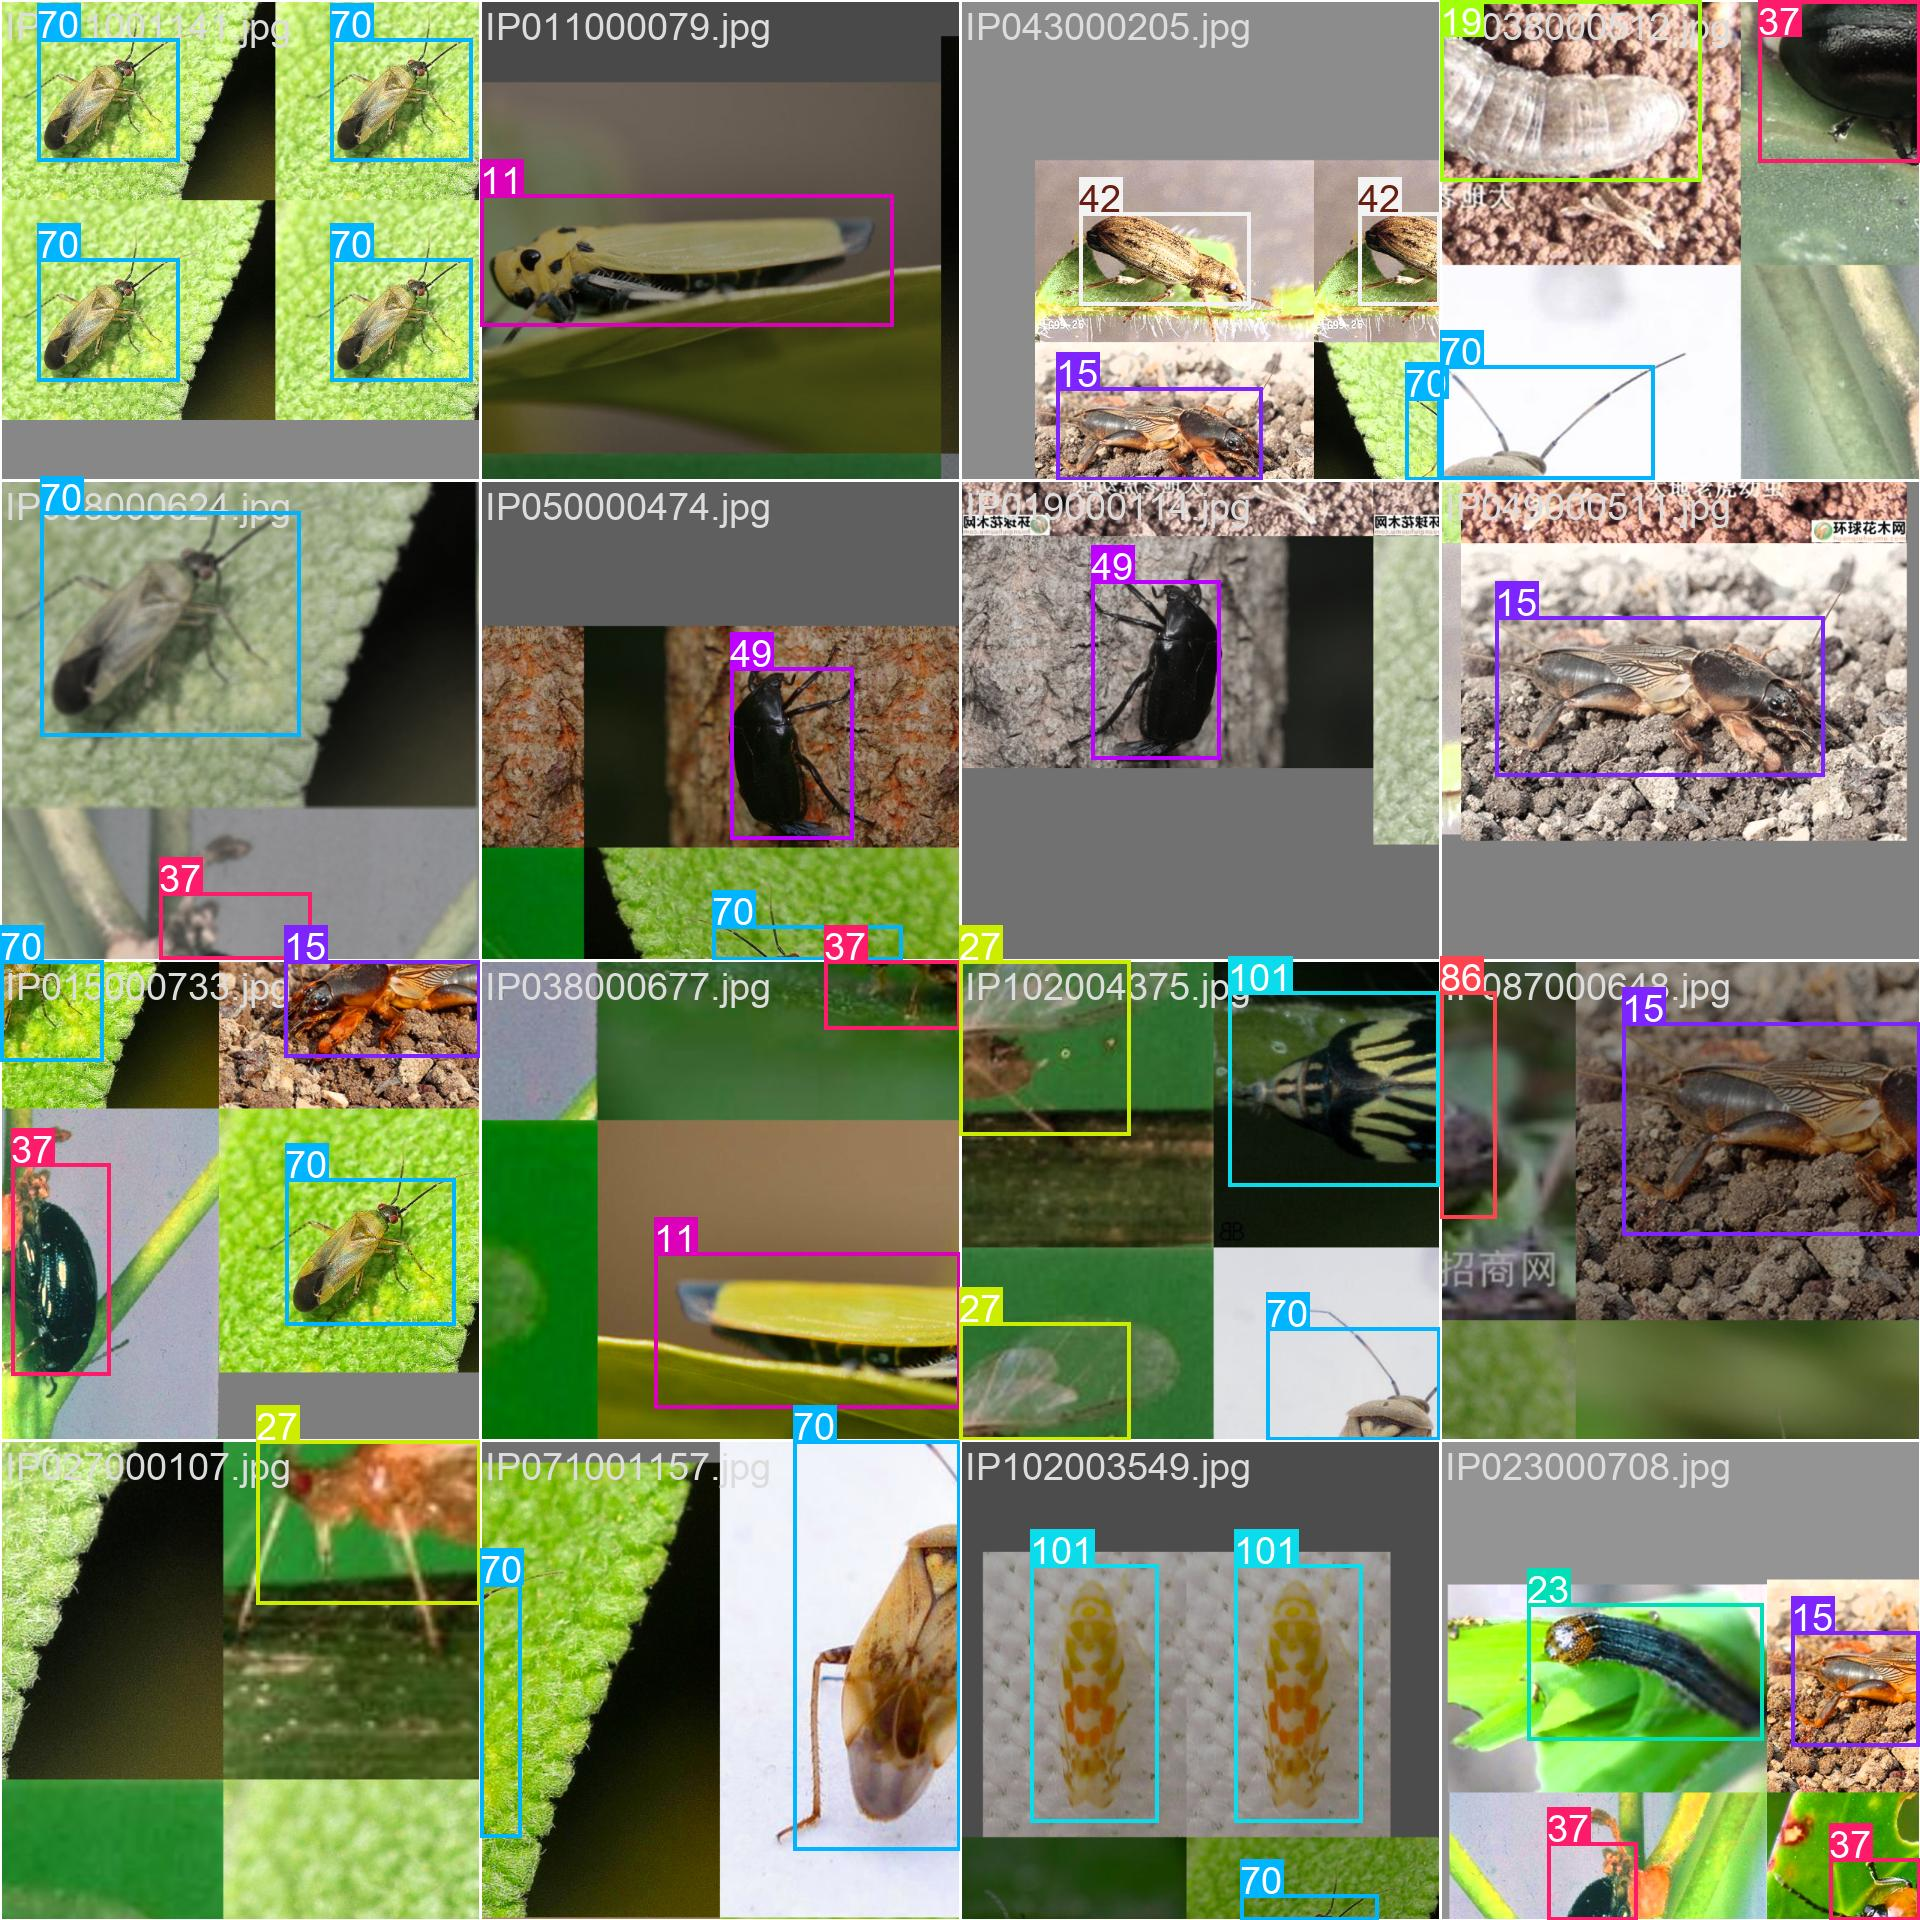
\includegraphics[width=0.8\columnwidth]{images/detection_results.png}
    \caption{Sample Detection Results on Test Images}
    \label{fig:detection_results_report}
\end{figure}

\subsection{Inference Speed}
Inference speed was evaluated on the web application using ONNX Runtime Web. The system achieved an average inference time of 45-60 ms per frame, corresponding to a processing speed of 16-22 FPS. This real-time performance is sufficient for interactive use and field deployment scenarios.

\section{System Implementation and User Interface}

\subsection{Web Application Interface}
The developed web application provides an intuitive interface for agricultural pest detection, featuring both pest detection and general object detection capabilities. Figure \ref{fig:ui_pest_detection_report} shows the pest detection interface, which allows users to upload plant images for automated pest identification.

\begin{figure}[H]
    \centering
    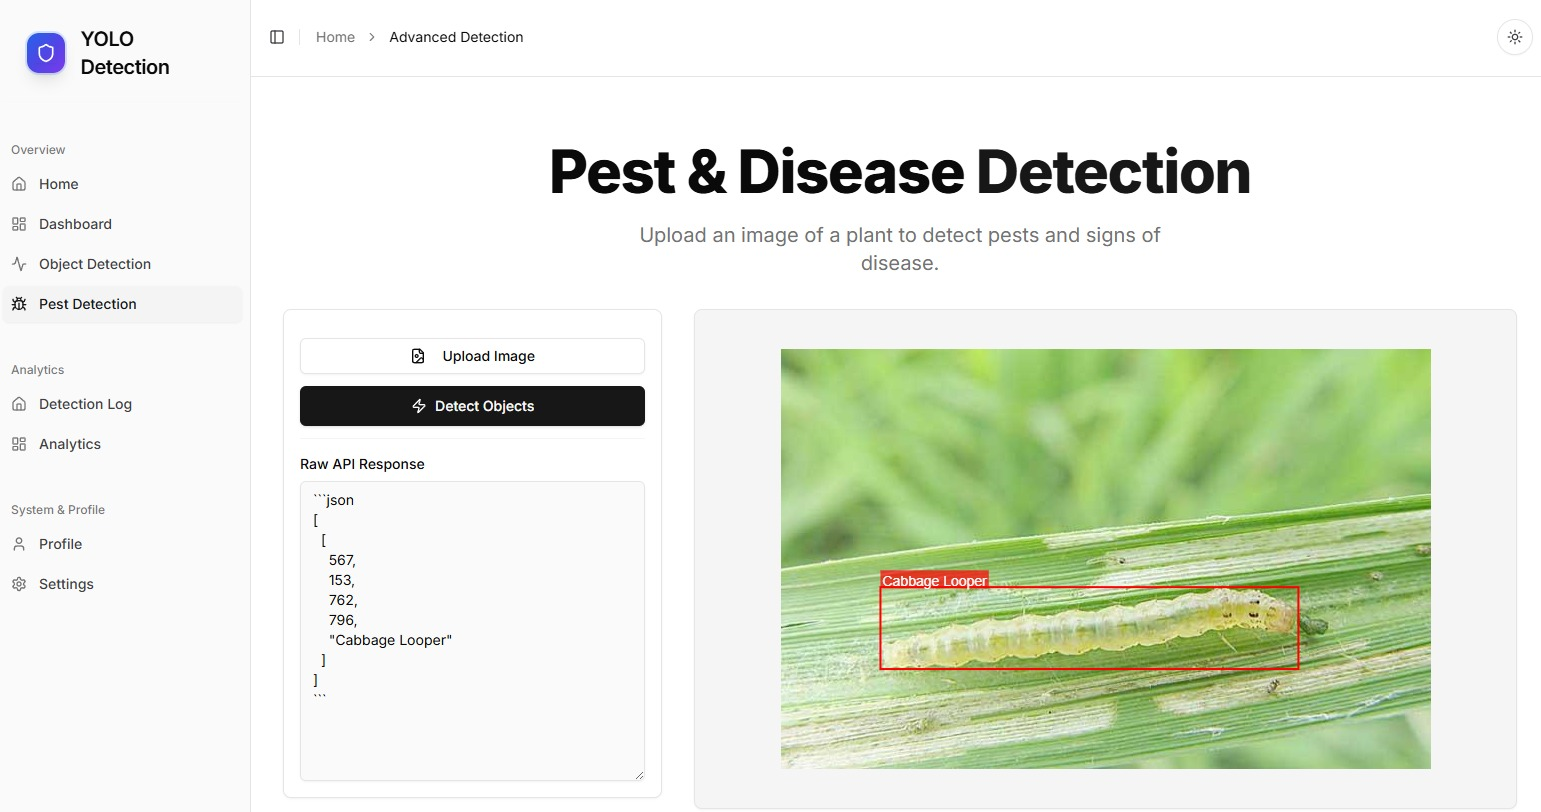
\includegraphics[width=0.8\columnwidth]{images/ui_pest_detection.png}
    \caption{Pest Detection Interface showing successful detection of Cabbage Looper with bounding box annotation and confidence score.}
    \label{fig:ui_pest_detection_report}
\end{figure}

The pest detection interface demonstrates the system's capability to accurately identify and localize agricultural pests within uploaded images. In the example shown, the system successfully detected a Cabbage Looper with precise bounding box coordinates and confidence metrics. The interface provides immediate visual feedback through bounding box overlays and detailed JSON response data for integration with other agricultural management systems.

\subsection{Object Detection Capabilities}
Beyond pest-specific detection, the system also incorporates general object detection capabilities as shown in Figure \ref{fig:ui_object_detection_report}. This expanded functionality allows for comprehensive monitoring of agricultural environments, detecting various objects that may impact crop health and management decisions.

\begin{figure}[H]
    \centering
    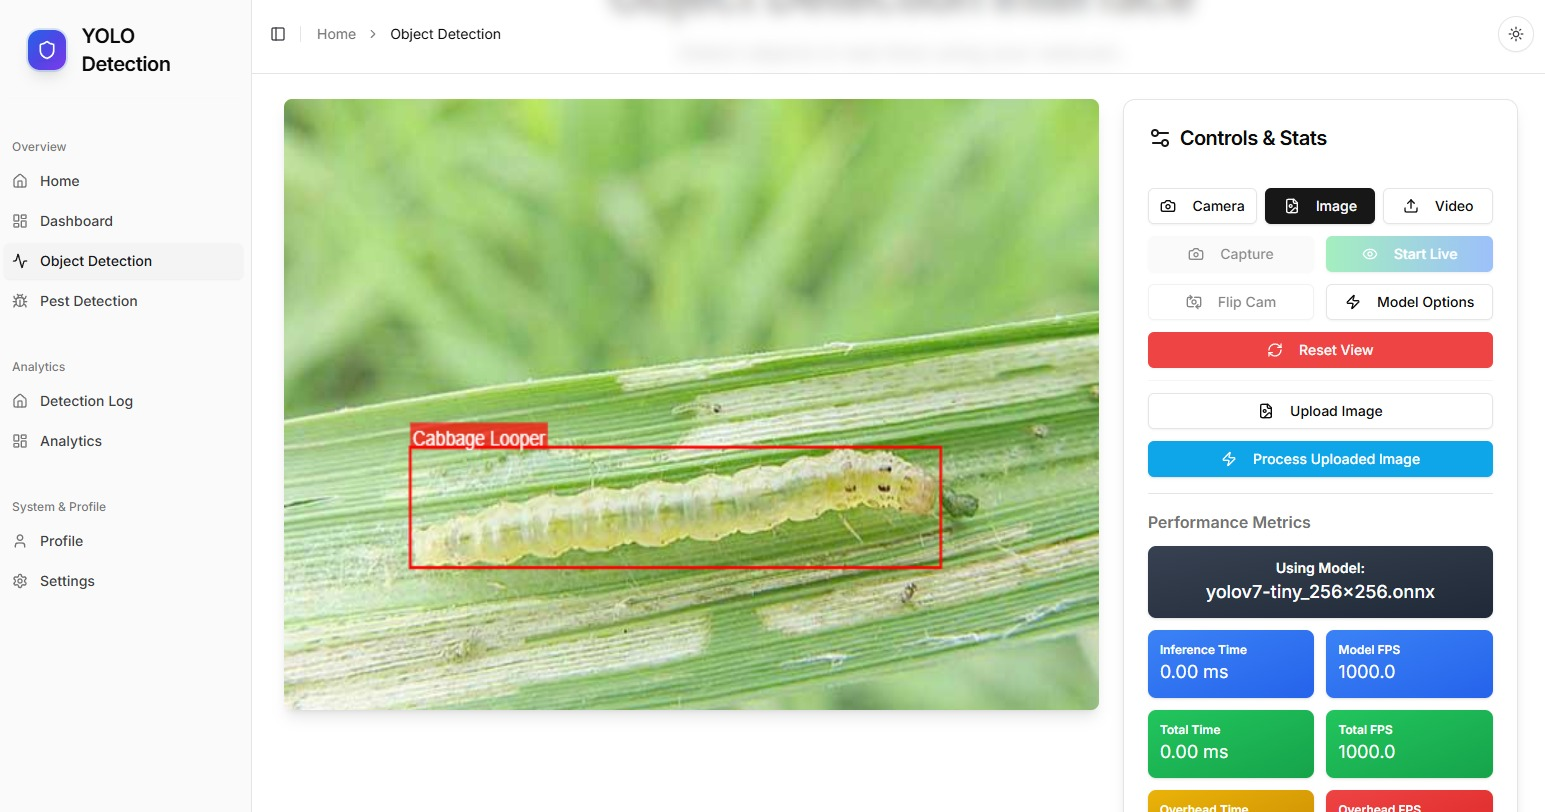
\includegraphics[width=0.8\columnwidth]{images/ui_object_detection.png}
    \caption{Object Detection Interface demonstrating the system's versatility in detecting various agricultural objects.}
    \label{fig:ui_object_detection_report}
\end{figure}

The object detection interface showcases the system's real-time processing capabilities with comprehensive performance metrics. Key features include live camera feed processing, model performance statistics (inference time, FPS), and flexible input options supporting camera, image upload, and video processing. The interface displays the current model configuration and provides real-time feedback on system performance, essential for field deployment scenarios.

\subsection{Technology Stack}
The application was developed using a modern technology stack to ensure performance, scalability, and maintainability. The key components are:
\begin{itemize}
    \item \textbf{Frontend Framework:} Next.js with React and TypeScript for building a robust and type-safe user interface.
    \item \textbf{Styling:} Tailwind CSS for a utility-first approach to styling, enabling rapid development of a responsive and modern UI.
    \item \textbf{Deep Learning Model:} A custom-trained YOLOv11 model, optimized for detecting a wide range of agricultural pests.
    \item \textbf{Web Inference Engine:} ONNX Runtime Web, which allows for high-performance model inference directly in the browser using WebAssembly.
    \item \textbf{Model Format:} The model is deployed in the optimized ONNX (.ort) format to minimize load times and maximize inference speed on the client-side.
\end{itemize}
